\documentclass{bioinfo}
\copyrightyear{2014}
\pubyear{2014}


\usepackage{hyperref}



\begin{document}
\firstpage{1}

\title[PconsFold]{PconsFold: Improved contact predictions improve
 protein models}
\author[M.Michel \textit{et~al}]{Mirco Michel\,$^{1,2}$, Sikander
  Hayat\,$^{3}$, Marcin Skwark\,$^{4}$, Chris Sander\,$^{5}$, Debora Marks\,$^{3}$,  and Arne Elofsson\,$^{1,2,}$\footnote{to whom correspondence should be addressed}}
\address{$^{1}$Department of Biochemistry and Biophysics, Stockholm University, 10691 Stockholm, Sweden, 
$^{2}$Science for Life Laboratory, Box 1031, 17121 Solna, Sweden, 
$^{3}$Department of Systems Biology, Harvard Medical School, Boston, Massachusetts, USA, 
$^{4}$Department of Information and Computer Science, Aalto University, PO Box 15400, FI-00076 Aalto, Finland, and
$^{5}$Computational Biology Center, Memorial Sloan-Kettering Cancer Center, New York, New York, USA}

\history{Received on XXXXX; revised on XXXXX; accepted on XXXXX}

\editor{Associate Editor: XXXXXXX}

\maketitle

\begin{abstract}

\section{Motivation:}
A few years ago it was noted that the quality of protein contact
predictions could be improved significantly if direct and indirect
information was separated and sufficient number of homologous
sequences are available. It was shown that the contact
predictions alone contain sufficient information to predict the
structure of many proteins. However, since the first reports there has
been improvements in the contact predictions methods. Further there
also exist slower, but potentially more accurate methods to model the
proteins. Here, we ask how much the final models are improved if (i)
improved contact predictions are used and (ii) if Rosetta is used to
model the proteins. 



\section{Results:}
Using the same 12 proteins as in the original publication of EVfold
the TM-score of the top ranked models are improved by on average 33\%.
We find that on average the quality is improved with about 15\% when
the improved contacts from plmDCA are used and another 16\% when
PconsC is used. Using Rosetta instead of
EVfold does not significantly improve global model accuracy. However,
the chemistry of models generated with Rosetta is improved.

\section{Availability:}
PconsFold is a fully automated pipeline for ab-initio protein
structure prediction based on evolutionary information. PconsFold is
based on PconsC contact prediction and uses the Rosetta folding
protocol. Due to its modularity, the contact prediction tool can be
easily exchanged. The source code of PconsFold is available on GitHub
at \url{https://www.github.com/ElofssonLab/pcons-fold} under the MIT
license.
\section{Contact:} \href{arne@bioinfo.se}{arne@bioinfo.se}
\section{Supplementary information:} Supplementary data are available at \emph{Bioinformatics} online.
\end{abstract}

\section{Introduction}
The protein folding problem is one of the longest standing problems in
structural biology. Although the problem itself remains largely unsolved,
there have been continuous effort and progress resulting in increased
accuracy of predicted models
\cite[]{kryshtafovych_CASP10_2013}. 

The idea of using predicted residue-residue contacts for protein
structure prediction is not new \cite[]{Vendruscolo9377713}. However,
until recently predicted contacts lacked the accuracy to facilitate
structure prediction methods significantly
\cite[]{marks_protein_2011}. This only became possible due to a new
approach to separate direct from indirect contact information
\cite[]{Weigt19116270,burger_disentangling_2010}. Since then there
has been continuous effort to improve the quality of predicted
contacts \cite[]{morcos_direct-coupling_2011, jones_PSICOV:_2012,
 ekeberg_improved_2013, skwark_PconsC:_2013}. In addition to the
initial predictions of soluble proteins \cite[]{marks_protein_2011}
and protein-complexes \cite{Schug20018738} now the predicted contacts
have also been applied in structure prediction of membrane proteins
\cite[]{hopf_three-dimensional_2012, nugent_accurate_2012}.


\begin{figure}[!tpb]%figure1
\centerline{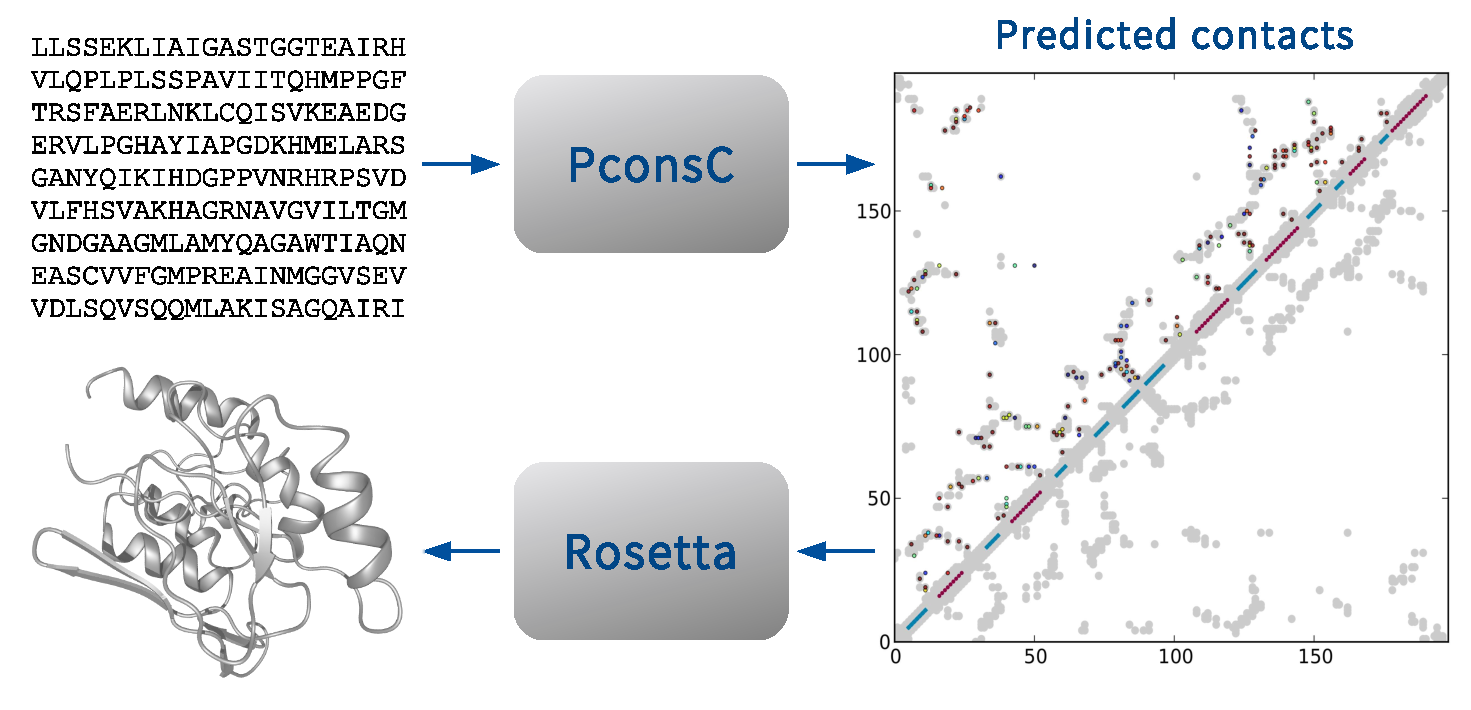
\includegraphics[scale=0.35]{figures/pipeline.eps}}
\caption{PconsFold pipeline. Based on a given protein sequence,
 amino-acid contacts are predicted with PconsC. These contacts then
 facilitate protein folding with Rosetta. In the end PconsFold
 outputs a structural model for the given
 sequence.}\label{fig:pipeline} 
\end{figure}

To optimize protein structure prediction from predicted contacts we
developed PconsFold, a pipeline for ab-initio protein structure
prediction of globular single-domain proteins
(Figure~\ref{fig:pipeline}). PconsFold is based on predicted
amino-acid contacts from PconsC. These contacts are utilized within
Rosetta to fold a given protein sequence from scratch. We benchmark
our method on two datasets and compare it to EVfold
\cite[]{marks_protein_2011}, a previous method for contact based
protein structure prediction. It was found that the improved quality of predicted contacts
by PconsC~\cite{skwark_PconsC:_2013} increases quality and
native-likeliness of predicted structures by about 33\% over the
original EVfold and 16\% over EVfold using the improved contact
predictions from plmDCA~\cite{ekeberg_improved_2013}.

\begin{methods}
\section{Methods}

\subsection{Datasets}
During the development of PconsFold we used the proteins from
\citeauthor{jones_PSICOV:_2012} \citeyear{jones_PSICOV:_2012} (PSICOV
dataset). The dataset consists of 150 single domain proteins with sequence
lengths between 52 and 266 amino acids. A list of all Protein Data
Bank (PDB) \cite[]{berman_protein_2000} and corresponding Uniprot
\cite[]{magrane_uniprot_2011} IDs is given in (Supplementary Table
1). 


For each protein we chose to use its PDB seqres sequence as input and
not its atom sequence. This avoids internal gaps due to missing
residues in the crystal structure. We chose not to use Uniprot
sequences directly due to mutations and other sequential differences
to the PDB sequences. This allows direct comparisons between predicted
models and native PDB structures. Taking account for structural
differences due to diverging sequences is thus not necessary. 

Due to technical reasons EVfold did not produce any models for the
protein 1JBE. 1JBE was therefore excluded from all evaluations.


As an additional comparison between PconsFold and EVfold we used the set
of 15 proteins as in \citeauthor{marks_protein_2011}
\citeyear{marks_protein_2011}. PDB and Uniprot IDs are given in
Supplementary Table 2. According to the Uniprot IDs we extracted the sequences from the
Pfam alignments that were used in the publication. These sequences were
submitted to the EVfold server and used as input for PconsFold.

\subsection{Contact prediction}
In case of PconsFold, residue contacts are predicted with PconsC
\cite[]{skwark_PconsC:_2013}. The contact predictor plmDCA
\cite[]{ekeberg_improved_2013} is used by Rosetta/plmDCA and
EVfold. Rosetta/plmDCA utilizes the direct output from plmDCA. In
EVfold predicted contacts are further optimized according to
\citeauthor{marks_protein_2011} \citeyear{marks_protein_2011}
(supplementary information). PSICOV was used in Rosetta/PSICOV. 


Predicted contacts were ranked according to the confidence score
assigned by the respective contact prediction method. For each protein
we selected $n = f \cdot l$ top-ranked contacts, where $l$ represents
the length of the protein sequence and $f$ a factor to scale $n$
relative to sequence length.



\subsection{Rosetta}
In PconsFold, Rosetta/plmDCA, and Rosetta/PSICOV we apply the
AbinitioRelax folding protocol \cite[]{rohl_protein_2004} of Rosetta
in version 2013wk42 \cite[]{leaver-fay_rosetta3:_2011}. The file {\tt
 abinitio.options\_tmpl} in the folder {\tt pcons-fold/folding/rosetta} of the GitHub
repository lists all options we are using with AbinitioRelax. 

We employ the function \emph{FADE} to integrate predicted residue
contacts into the internal scoring function of Rosetta. \emph{FADE}
calculates the energy of a given contact as a function of the distance
$d$ between its residues as given by the following equation:

\begin{equation}%\label{eq:fade}
\textit{FADE}(d) = \left\{
\begin{array}{l l l}\label{eq:fade}
%2b_{low}^3 - 3b_{low}^2 + 1 & \quad \textrm{if d $<$ $c_{low}$} \\
%2b_{up}^3 - 3b_{up}^2 + 1 & \quad \textrm{if d $>$ $c_{up}$} \\
0.0 & \quad \textrm{for $d < lb$ or $d > ub$} \\
-2(\frac{d - \textit{lf}}{z})^3 - 3(\frac{d - \textit{lf}}{z})^2 + 1 & \quad \textrm{for $d < \textit{lf}$} \\
2(\frac{d - \textit{uf}}{z})^3 - 3(\frac{d - \textit{uf}}{z})^2 + 1 & \quad \textrm{for $d < \textit{uf}$} \\
w & \quad \textrm{otherwise.} \\
\end{array} \right.
\end{equation}

The parameters $lb$ and $ub$ are lower and upper bounds, $z$
represents the fading zone's width, $\textit{lf}$ and $\textit{uf}$
denote the inner boundaries for the fading zone $lb + z$ and $ub - z$,
respectively. The well-depth of the interval between both inner
boundaries is given by $w$. We set $lb$ to -10 \AA, $ub$ to 19 \AA\
and $z$ to 10 \AA. This defines a contact to be fully formed if the
participating residues are within 9 \AA\ of each other. The fading
zones allow for a soft margin between formed and non-formed
contacts. In terms of energy all non-formed contacts are ignored. In
our opinion this accounts best for the fuzzy nature of predicted
contacts. The fading zone at the lower bound allows Rosetta to detect
and resolve overlapping residues, i.e. when there is a negative
distance between two residues. 

\subsection{EVfold}
On the PSCOV dataset EVfold was run in a standalone version. The alignment E-value cutoff was fixed to $10^{-4}$. The parameter $m$ was set to 0.9. This defines a threshold to exclude sequences from the alignment that consist of more than 90\% of gaps. This was done to enable comparison with other methods. In general EVfold choses E-values based on sequence coverage and number of sequences found.

The current web server version of EVfold was run with default parameters on the small test set. We ensured that it uses plmDCA instead of DCA for contact prediction.

\subsection{Identification of top ranked model}

In addition to internal Rosetta scoring we assessed the quality of all
predicted models with the model quality assessment programs (MQAPs)
Pcons \cite[]{lundstrom_pcons:_2001}, ProQ2
\cite[]{ray_improved_2012}, and DOPE from the Modeller software
package \cite[]{eswar_comparative_2006}. Pcons uses a comparative
approach and ranks all decoys according to pairwise structural
similarity between them. ProQ2 and DOPE assess single proteins and
evaluate structural features, such as side-chain placement and overall
shape. For our ranking we use the global score each MQAP assigns to a
predicted structural model (decoy). Residue-wise information about
local model quality is not used. 

For each structure prediction method all decoys were re-ranked with
each MQAP. The top-ranked model was then selected and compared to its
native structure. For this comparison we used the TM-score
\cite[]{zhang_scoring_2004} as a measure of structural similarity. As
native structure we used the PDB structure of each protein without
further loop-closing or other refinement. Tags from seqres
sequences, although modeled, are therefore ignored in the structural
comparison.

The positive predictive value (PPV) was calculated to assess the quality of predicted models. It indicates how well a given contact map fits a given structure. All PPV values were calculated using reference contacts C$^{\beta}$ (C$^{\alpha}$ in case of glycine) distances in the structure (native or model) with a cutoff at 8 \AA\.


\subsection{Model quality assessment}

We used MolProbity \cite[]{chen_molprobity:_2010} to assess the chemical
model quality. The MolProbity tool {\tt oneline-analysis} was used to 
detect clashes and to evaluate backbone dihedrals as well as 
side-chain rotamers. To prepare all structures for this analysis, we 
first relaxed them with fixed backbone atoms.
The Rosetta protocol {\tt relax.linuxgccrelease} was used with the flags 
{\tt -relax:quick} {\tt -in:file:fullatom} {\tt 
-constrain\_relax\_to\_start\_coords}. Hydrogen atoms were then 
added with the MolProbity tool {\tt reduce-build}. All resulting 
structures are provided in the Supplementary Material.



\subsection{Running time}
A reduction from 20,000 to 2,000 decoy structures corresponds to a 10-fold
decrease of runtime during the Rosetta folding step but also leads to an
expected decline in average model quality. On one core of an Intel
E5-2660 (2.2 GHz Sandybridge), the calculation of one decoy takes
between 1 and 10 minutes for the shortest and longest protein in the
PSICOV dataset respectively. To compute 2,000 decoys for each protein
we ran 16 threads in parallel. Each of these threads then generates
125 decoys, starting with independent random seeds. With this setting
it takes between two hours and nearly one day to generate all decoys
for one protein. This simple scaling is possible since Rosetta runs
are independent of each other as long as they are based on 
independent random seeds. Increasing the number of threads can then be used to reduce
overall runtime or to generate more decoys within a given timespan.

\end{methods}


\section{Results and Discussion}

\subsection{PconsFold}

\begin{figure*}[!tpb]%figure1
\centerline{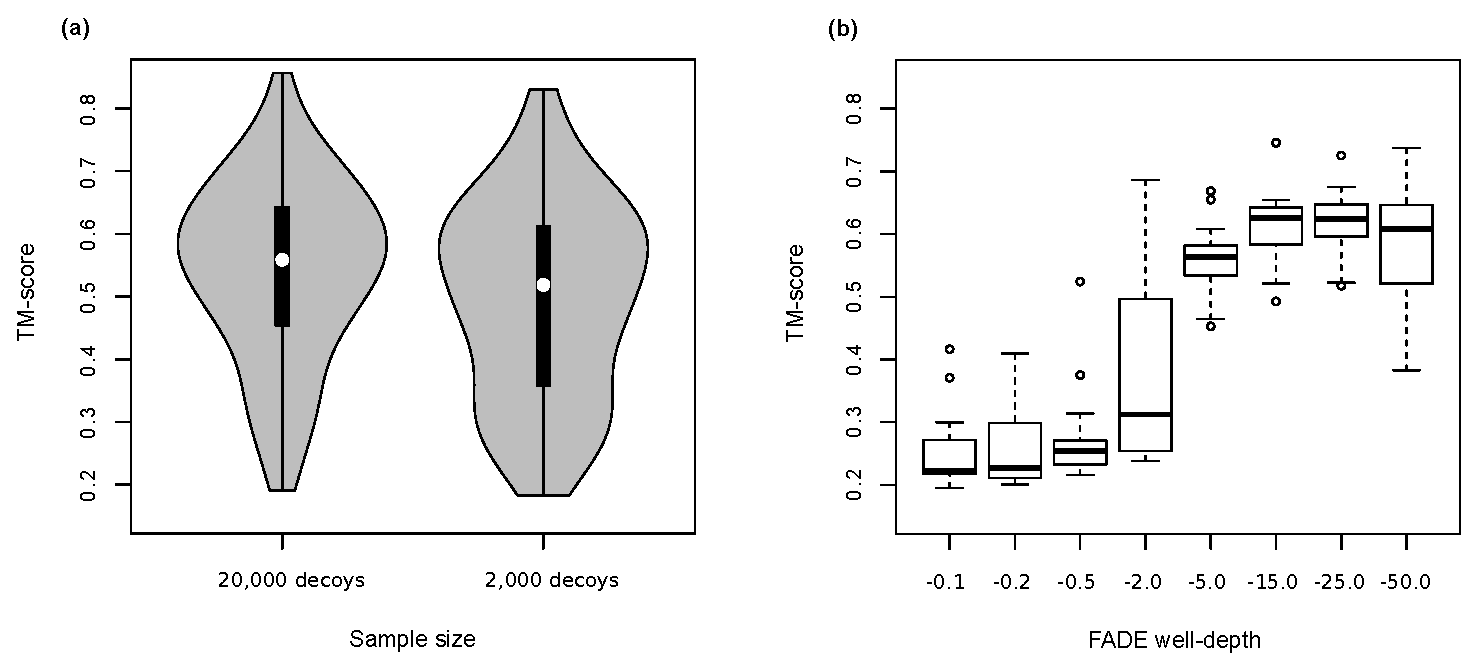
\includegraphics[scale=0.7]{figures/rosetta.eps}}
\caption{Model quality in TM-score for adjustments of two
 different Rosetta parameters. (a) Performance distributions 
 for two different sample sizes of 20,000 (left) and 2,000 (right) 
 decoy structures. The black boxes indicate upper and lower 
 quartile with white dots at the median of the distributions. For each 
 protein in the full PSICOV dataset the top 
 ranked model was selected from the decoys by its Rosetta score and 
 compared to the native structure. (b) Effects of adjustments to 
 the well-depth parameter of the FADE function. A low absolute 
 well-depth (left side) puts low weight on predicted constraints. 
 Constraints are stronger weighted by higher absolute values of 
 well-depth (right side). A subset of 14 proteins of the PSICOV dataset was used here.}\label{fig:ros} 
\end{figure*}

For all results in this section, we used the internal Rosetta score to
rank all predicted decoys. The top-ranked decoy structure was then
selected as a final model. With the {\tt -nohoms} flag during fragment
picking we ensured that all homologous structures are excluded. Only
fragments from non-homologous protein structures were selected. This
was done to simulate a real application case and not to overestimate
prediction performance. If not stated otherwise, we used all 150 proteins of
the PSICOV dataset as prediction targets in this section. 

Previous studies have shown that 20,000 -- 200,000 decoys are
necessary to sample native-like conformations without using spatial
constraints \cite[]{Simons10526365}. We set out using 20,000 models
and then reduced the number of decoy structures to
2,000. The bulk at around 0.3 TM-score in the second
distribution of Figure~\ref{fig:ros}(a) represents an increased
number of low quality models. We think the practical advantages of
massively shorter Rosetta runs outweigh slightly worse predicted
models. This parameter is therefore set to a default value of 2,000
but can be specified by the user via a command line argument. All
further results in this section are generated with this default
setting. 


We selected the FADE function to incorporate predicted residue
contacts into Rosetta's native energy function. We then adjusted the
parameter $w$ (well-depth) of FADE (Equation~\ref{eq:fade}) on a
subset of 14 Proteins (Supplementary Table 1, marked with asterisk) of the PSICOV
dataset. The resulting TM-scores are shown in Figure~\ref{fig:ros}(b). The energy term from spatial constraints diminishes with
well-depth values of -0.5 and above. This leads to a significant
decrease in model quality. Lower values of -5.0 and below put a larger
absolute weight on the constraints resulting in higher model
qualities. We assume this is due to the small number of decoys we are
generating in this experiment. Without the help of spatial 
constraints Rosetta's internal energy function does not converge. 
At the end we choose to use a value of -15.0 to achieve
high model quality without outweighing Rosetta's internal energy
function completely.


\begin{figure*}[!tpb]%figure1
\centerline{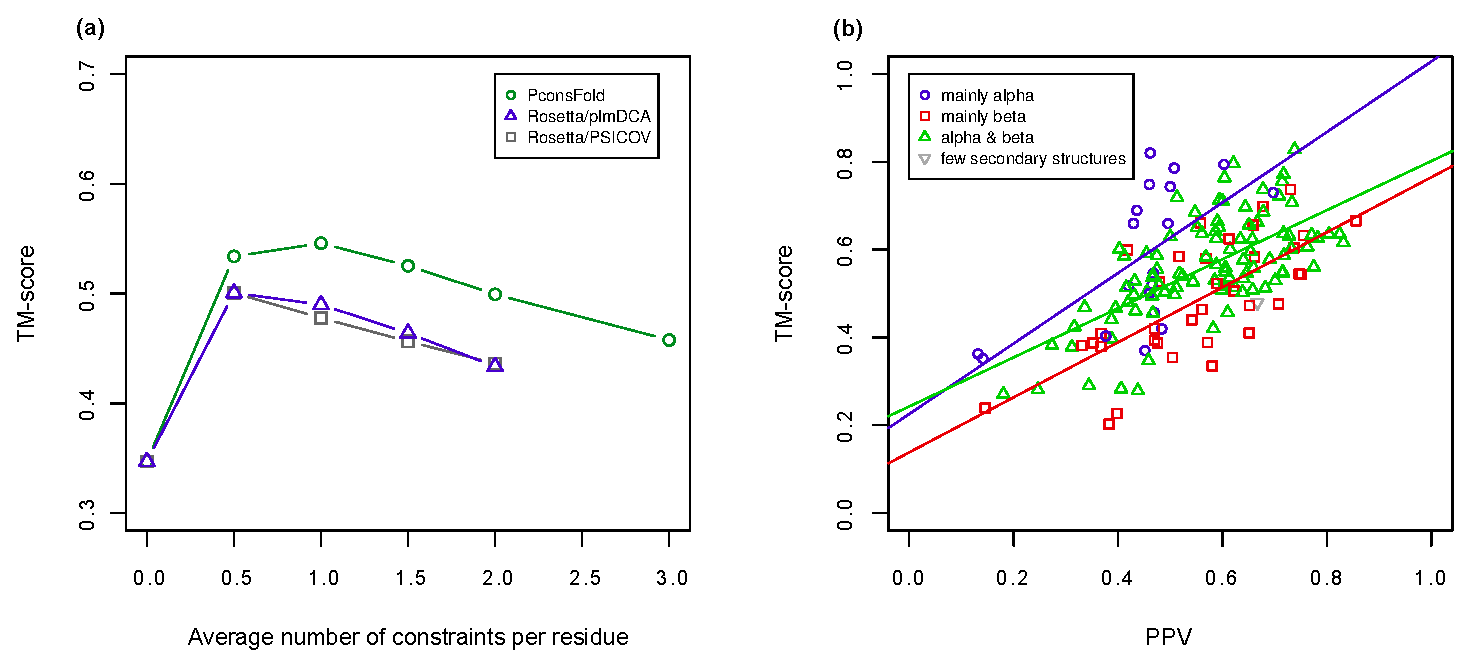
\includegraphics[scale=0.7]{figures/tmscores.eps}}
\caption{Folding performance on the full PSICOV dataset. (a) The 
 number of contacts used in structure prediction is
 plotted against average TM-score for three different methods:
 PconsFold (green circles), Rosetta/plmDCA (blue triangles), and
 Rosetta/PSICOV (black squares). For each protein the number of top
 ranked contacts was selected relative to its sequence length. A value
 of 1.0 on the $x$-axis represents one
 contact per residue on average. b) TM-scores are compared
 to the PPV of underlying contact maps for PconsFold (using
 PconsC). The colors represent all four CATH fold classes. Lines 
 are fitted to the data to illustrate performance differences between the fold classes.}\label{fig:main}
\end{figure*}

With any number of contacts used during structure prediction, the
resulting model quality is on average higher than it would be without
contact information. Comparing $x=0.0$ to any
other $x$ in Figure~\ref{fig:main}(a) shows that predicted contacts generally improve model
quality, regardless of method or amount of contacts. 


Improvements in contact prediction methods also increase the quality
of predicted structures. With a maximal average TM-score of 0.55
PconsFold, i.e. using PconsC contacts, provides a 10\% improvement
over using PSICOV or plmDCA contacts. This observation is consistent
with a direct comparison of contact prediction methods as in
\citeauthor{skwark_PconsC:_2013}
\citeyear{skwark_PconsC:_2013}. However, the performance difference
between PSICOV and plmDCA diminishes when their contacts are used in
structure prediction. 


There is an optimal number of contacts, specific to the contact
prediction method. In Figure~\ref{fig:main}(a) the maximal average
TM-score is reached at $x=1.0$ for PconsFold. For Rosetta/PSICOV and
Rosetta/plmDCA a smaller number than one contact for every residue 
is optimal. This can also be explained by the quality of
predicted contacts. A larger number of top ranked contacts is
predicted with a higher quality in PconsC compared to plmDCA or PSICOV
\cite[]{skwark_PconsC:_2013}. Using more of these contacts during
structure prediction leads to improved models. 


This relation between contact and model quality can also be observed
in Figure~\ref{fig:main}(b).The overall Pearson correlation between PPV and TM-score in
this dataset is 0.59. Proteins with contact maps of lower quality tend
to be modeled less accurate. 


Proteins belonging to the {\it
 mainly alpha} CATH fold class seem to be easier to fold than
proteins from the {\it alpha \& beta} fold class and proteins from the
{\it mainly beta} fold class seem to be hardest to fold. The fold
classes are indicated by the color scheme in Figure~\ref{fig:main}. Predicted contact maps in mainly $\alpha$-helical proteins (blue)
have similar or lower PPV values than those of $\beta$-sheet
containing proteins (green and yellow), but the resulting models are
more accurate in terms of TM-score.




\subsection{Identification of top ranked model}
Table~\ref{tab:qa} summarizes the evaluation of different MQAPs on the
predictions for the PSICOV dataset. It shows average TM-scores for
top-ranked models after re-ranking all models with each MQAP. In all
cases the cumulative score for the full protein was used. Due to
technical reasons, Rosetta's internal scoring function was not
applicable to the models generated by EVfold. For PconsFold and
Rosetta/plmDCA the internal scoring was able to pick the best model on
average. In case of EVfold, Pcons selected the best models on
average. Pcons performed slightly worse than the internal scoring
function of Rosetta on the models from PconsFold and
Rosetta/plmDCA. ProQ2 did not perform well on EVfold models. ProQ2 performed slightly worse than
Pcons on models from PconsFold and Rosetta/plmDCA. We also tested a
combination of both, as in \citeauthor{wallner_pcons.net:_2007}
\citeyear{wallner_pcons.net:_2007}. However, the results are omitted
since they were not significantly different from those of Pcons
alone. DOPE scoring of EVfold models worked almost as good as Pcons,
but we observe a strong decline in average model quality for PconsFold
and Rosetta/plmDCA. We assume Rosetta scoring performed best, because predicted contacts
are part of the energy function. Models that satisfy predicted
contacts most optimally are assigned low energies and thus ranked on top.

\begin{table}[!t]
\processtable{Average TM-scores for top-ranked models selected by different MQAPs. \label{tab:qa}}
{\begin{tabular}{llll}\toprule
Method & EVfold & PconsFold & Rosetta/plmDCA \\ \midrule
Rosetta & -- & 0.55 & 0.50 \\
Pcons & 0.47 & 0.53 & 0.47 \\
ProQ2 & 0.36 & 0.51 & 0.46 \\
DOPE & 0.46 & 0.36 & 0.32 \\ \botrule
\end{tabular}}{}
\end{table}

\begin{figure*}[!tpb]%figure1
\centerline{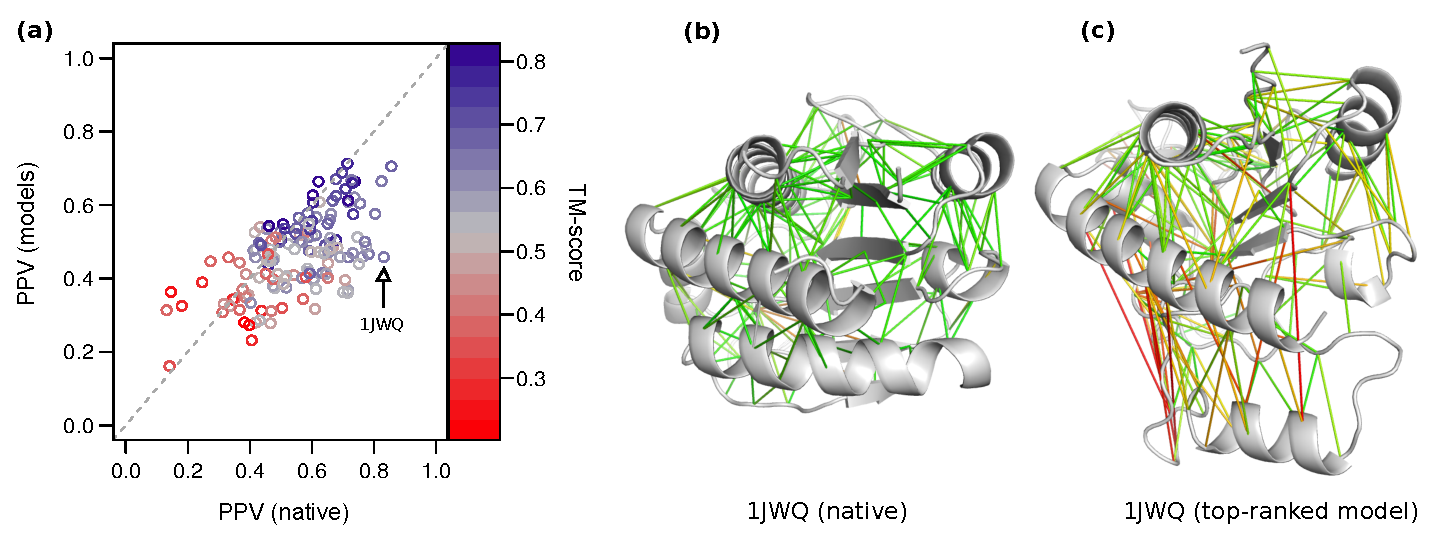
\includegraphics[scale=0.7]{figures/qa.eps}}
\caption{Analysis of contact maps in native structures and
top-ranked models. PPVs were calculated for the sets of contacts that
were used during folding ($1.0 \cdot l$ top-ranked contacts) with a
C$^\beta$ distance cutoff of 8~\AA\ in the structures. (a) PPV values for PconsC contacts on native structures 
($x$-axis) against PPVs on the top-ranked models from PconsFold 
($y$-axis). The colors represent TM-scores of models against native
structures. (b) Native structure of 1JWQ. Lines represent all predicted contacts. The color 
scheme indicates spatial distances of residue pairs in the 
structure. The PPV is 0.83. (c) Predicted contacts in the top-ranked 
model for 1JWQ with the same color scheme. This model has a TM-score 
of 0.62 and a PPV of 0.46}\label{fig:qa}
\end{figure*}

With an average of 0.55 the
PPV of predicted contacts is higher in native structures than in the models, which have an
average PPV of 0.47. The points in the lower right
triangle in Figure~\ref{fig:qa}(a) indicate room for further improvement
of the folding process. In the region around PPV 0.4 and below,
some models satisfy the constraints better than the native
structures. A PPV of 0.4 means that 60\% of the predicted contacts 
are false positives. We assume that such low quality contact maps
mislead the structure prediction process. This results in models that
diverge from native structures with a better fit to the predicted
contacts. 


In Figure~\ref{fig:qa} (b) and (c) we examine one example of
non-optimal folding more closely. We selected 1JWQ since it 
represents the worst-case scenario where the difference between 
native and model PPV is largest. The lines represent predicted 
contacts, colored according to the distance between their C$^{\beta}$
atoms. In case of glycine C$^{\alpha}$ atoms are used instead. The
color gradient indicates distances ranging from 4 \AA\ in green over
yellow at 10 \AA\ up to red for 20 \AA\ and above. With a PPV of
0.83 most of the contacts were predicted correctly for this
protein. This results in mainly green colored contacts in the native
structure in (b). Looking at the contacts in (c) reveals that the
helix at the bottom was not optimally packed in the model. Contacts
colored in orange and red show that the distance constraints were not
sufficiently satisfied by Rosetta. The overall PPV decreased to 0.46
for this model.







\subsection{Comparison to EVfold}

When looking at Figure~\ref{fig:vs} the majority of alpha helical
proteins (blue) achieved higher TM-scores with PconsFold than with
EVfold. On average we see an improvement of 14\% of PconsFold over
EVfold on alpha helical proteins. The same improvement can also be
observed for Rosetta/plmDCA. Together with Figure~\ref{fig:main},
this indicates that Rosetta performs better on alpha-helical
proteins. Further investigation is needed to see if this trend is
merely due to a bias in the underlying dataset. The average
performance of PconsFold on alpha \& beta proteins (green) is 15\%
higher than for EVfold. However, Rosetta/plmDCA performs equally good
as EVfold on average on such targets. The improvement might thus be
due to PconsC contact maps, since it is only observable for PconsFold
and not for Rosetta/plmDCA. At a level of single proteins we see quite
some divergence between the results of EVfold and PconsFold in
Figure~\ref{fig:vs}. This is especially true for ``mainly beta''
proteins and ``alpha \& beta'' as well as ``mainly beta''.

The analysis with MolProbity reveals that the backbone dihedral
quality of Rosetta models is higher than for EVfold models. The
percentage of Ramachandran outliers is 0.62\% for PconsFold and 12.16\% for EVfold. MolProbity further reports an average clash score of
10.48 for PconsFold and 9.90 for EVfold. The EVfold models have
slightly less clashes than the models from PconsFold. The average
final MolProbity score is with 1.85 better for PconsFold then 2.38 for
EVfold. This corresponds to a better average MolProbity percentile
rank of 80.69 for PconsFold than the average rank of 54.21 for EVfold.


Table~\ref{tab:evfold} contains TM-scores for the top-ranked models of
each protein in the small test dataset. We compare the EVfold results,
as published in \citeauthor{marks_protein_2011}
\citeyear{marks_protein_2011}, with results from the current EVfold
version (web) and PconsFold with 20,000 generated decoys. The results
for the current version of EVfold were generated using plmDCA instead
of DCA as in the published version. With an average TM-score of 0.55
EVfold using plmDCA performs 15\% better than EVfold with DCA,
showing the importance of improved contact prediction. When using
PconsFold there is an additional improvement of 16\% to an average
TM-score of 0.64. This further supports our assumption that improved
contact maps improve structure prediction.

\begin{figure*}[!tpb]%figure1
\centerline{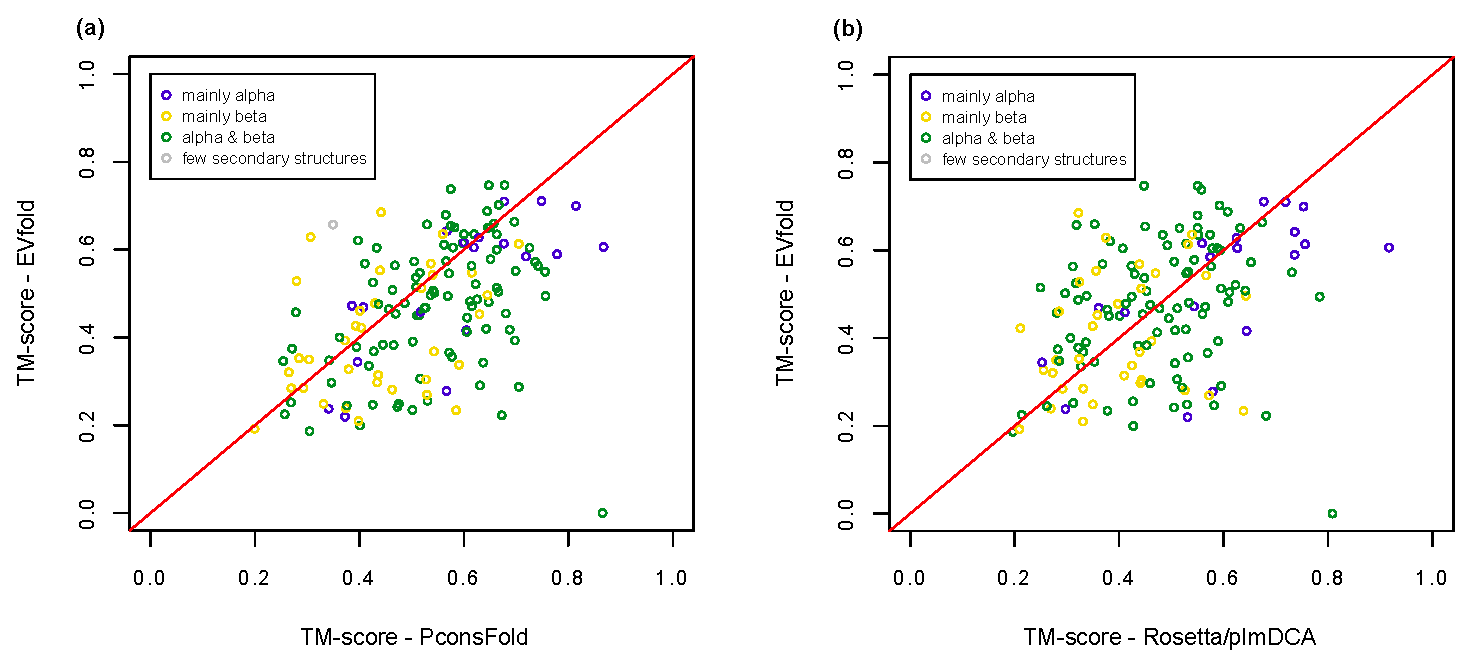
\includegraphics[scale=0.7]{figures/vs.eps}}
\caption{TM-score comparison for top-ranked models of the proteins in
 the PSICOV dataset. The decoys for each method were re-ranked using
 Pcons to assess the performance of the structure prediction process
 independent of the model ranking scheme. The colors represent all
 four CATH fold classes. (a) PconsFold compared to EVfold. (b)
 Rosetta/plmDCA compared to EVfold.}\label{fig:vs}
\end{figure*}

\begin{table}[!t]
\processtable{TM-scores for top ranked models comparing EVfold as it
 was published, current EVfold server (accessed Feb. 2014), and
 PconsFold with 20,000 decoys. \label{tab:evfold}}
{\begin{tabular}{lp{1.5cm}p{1.5cm}p{1.5cm}p{1.5cm}}\toprule
Protein & EVfold (paper) & EVfold (web)  & PconsFold\\\midrule
BPT1\_BOVIN & 0.49 & 0.25  & 0.57 \\
CADH1\_HUMAN & 0.55 & 0.54  & 0.53 \\
CD209\_HUMAN * & 0.39 & 0.64  & 0.54 \\
CHEY\_ECOLI & 0.65 & 0.66  & 0.82 \\
ELAV4\_HUMAN & 0.57 & 0.61  & 0.80 \\
O45418\_CAEEL & 0.48 & 0.62  & 0.65 \\
OMPR\_ECOLI & 0.35 & 0.44  & 0.59 \\
OPSD\_BOVIN & 0.50 & 0.55  & 0.56 \\
PCBP1\_HUMAN & 0.25 & 0.43  & 0.60 \\
RASH\_HUMAN & 0.70 & 0.62  & 0.67 \\
RNH\_ECOLI & 0.54 & 0.66  & 0.61 \\
SPTB2\_HUMAN & 0.37 & 0.51 & 0.74 \\
THIO\_ALIAC & 0.55 & 0.56  & 0.83 \\
TRY2\_RAT & 0.53 ** & 0.78  & 0.54 \\
YES\_HUMAN & 0.35 & 0.31  & 0.57 \\ \midrule
Mean & 0.48 & 0.55  & 0.64 \\ \botrule
\end{tabular}}{* The Uniprot entry A8MVQ9\_HUMAN of the EVfold publication was renamed into CD209\_HUMAN. ** This value was corrected as in the original publication it showed the value for the best possible model.}
\end{table}


\section{Conclusion}

Here, we show that improved contact predictions from
PconsC~\cite{skwark_PconsC:_2013} actually lead to improvements in
protein structure prediction. Further, it is clear that for proteins
with better-predicted contacts the generated models are of higher
quality, i.e. future improvements in contact predictions will result
in higher quality models. A comparison between using Rosetta and
EVfold indicates that using similar contact predictions generates
models of similar quality. However, Rosetta models are chemically
more correct. Finally, it is also clear that in many top ranked models
the contacts are less well satisfied than in the native structures,
i.e. an improved folding protocol would improve the models. One
option would be to use model-PPV as a measure of model quality, or as
a stopping criterion for decoy generation.



\section*{Acknowledgement}
Joel Hedlund is acknowledged for technical advice and valuable contributions to the code. 

\paragraph{Computational resources\textcolon}
The computations were performed on resources  at PDC Centre for High Performance Computing (PDC-HPC) and on resources provided by SNIC through Uppsala Multidisciplinary Center for Advanced Computational Science (UPPMAX) and National Supercomputer (NSC) Centre in Linköping, Sweden. 

\paragraph{Funding\textcolon}
This work was supported by grants from the Swedish
Research Council (VR-NT 2012-5046, VR-M 2010-3555), SSF (the Foundation for
Strategic Research) and Vinnova through the Vinnova-JSP program, and SeRC the
Swedish E-science Research Center. SH was supported by a R01 grant to
DS and CS.

\bibliographystyle{natbib}
%\bibliographystyle{achemnat}
%\bibliographystyle{plainnat}
%\bibliographystyle{abbrv}
%\bibliographystyle{bioinformatics}
%
%\bibliographystyle{plain}
%
\bibliography{pcons_fold}



\end{document}

